\documentclass[twoside]{IEEEtran}
\title{Supervised Machine Learning for \\ Color Classification}
\author{Benjamin~Hall}
\date{2023, March 20}
\markboth{}{Hall: Supervised Machine Learning for Color Classification}

\usepackage[bookmarksnumbered, hidelinks, colorlinks, allcolors=, urlcolor=blue]{hyperref}
\usepackage{url}

\usepackage{mathtools}
\interdisplaylinepenalty=2500

\usepackage{booktabs}

\usepackage{graphicx}
\usepackage[caption=false,font=footnotesize]{subfig}
\usepackage{stfloats}

\begin{document}
\maketitle

\begin{abstract}
    Color classification is typically achieved using hand-tuned algorithms. However, the algorithms generally need to be
    retuned when the environment changes, and the simple boundaries produced may not be sufficiently accurate. This study
    analyzes the effectiveness of using supervised machine learning to replace these traditional algorithms. The k-nearest
    neighbor, Bayesian linear classifier, and multiclass single-layer perceptron (SLP) algorithms were tested. Additionally,
    the colors were tested in both the RGB format and the complex HSV format, where numbers on the complex unit circle are
    used to represent hue. Results show that a multiclass SLP, adjusted to support complex numbers, can most accurately and
    efficiently classify colors, and the complex HSV format outperforms RGB with the data tested.

    Further research is needed to prevent the SLP algorithm from entering a local minimum, as well as to compare its
    accuracy on the RGB and complex HSV formats with more advanced color groups, such as classifying into various
    categories of blue.
\end{abstract}

\section{Introduction}

\IEEEPARstart{C}{olor} classification is used extensively in robotics and image processing. Companies use it to
automate the detection of certain product defects. Autonomous vehicles use color classification
to help detect road signs, determine the color of a traffic light, and so on. FIRST robotics teams
use color detection for vision targeting and autonomous robot operations.

Color classification can be done with fairly reasonable accuracy using image processing and
fairly simple algorithms, such as checking if the HSV values of a color are within a certain
range. However, the image processing can be an expensive operation, and the simple algorithms
often need to be retuned if the environment changes, such as with new lighting. Additionally, the
algorithms typically only target one or two colors, as hand-tuning the algorithm becomes more
time-consuming and prone to error as the list of colors grows. Furthermore, the algorithms often
draw simple, rectangular boundaries between color classifications.

AI provides an alternative method of color classification. Rather than relying on hand-tuning of
algorithms whenever the environment changes and dealing with human error, an AI based on
supervised machine learning can efficiently tune an algorithm to identify colors given enough
training data. This can result in massive time savings, as humans now only need to collect data
samples to feed the AI, and it has the potential to increase the accuracy of the algorithm, as it can
create advanced, mathematically optimized classification boundaries.

\section{Technical Discussion}

When it comes to supervised machine learning, there are three fairly simple algorithms that stand
out: k-nearest neighbors, the Bayesian linear classifier, and the single-layer perceptron algorithm.

k-nearest neighbors is a very simple algorithm to implement and can handle non-linear
classification boundaries. The algorithm calculates the distance between the test data point and
each training data point, and then it partial sorts those distances until it has the n closest
neighbors. The data gets whichever classification is most prominent among those neighbors.
However, the algorithm slows down as the training data set grows, as both calculating the
distances and performing the partial sort take linear time relative to the size of the training data.
The algorithm also has a high memory cost, as it needs to keep the training data in memory
during the entire program runtime to perform the partial sort.

The Bayesian linear classifier fixes both the time and memory costs by calculating ahead of time the
mean vectors of the classifications. The algorithm only needs to keep a vector of classification means
during program runtime, and classifying a test data point is simple: for each classification, take
the dot product of the data point with the classification's mean vector and add the result of the
classification's mean vector dotted with itself. The data point then gets the classification with the
largest output. However, the algorithm assumes a linear boundary between classifications, and it assumes
that the data's class conditional density functions follow a Gaussian distribution~\cite{farmer}, which
is often not the case.

The single-layer perceptron algorithm relaxes the assumption of a Gaussian distribution to
provide a more general linear classifier. Instead of using a vector of means, the algorithm trains a
vector of weights by testing the training points against the weights, calculating the error, and
adjusting the weights accordingly. In its simplest form, the SLP only splits data into two
classifications using a linear boundary and a single vector, assigning positive outputs to one class
and negative outputs to another. However, the algorithm can also be generalized into a multiclass
algorithm by storing weight vectors for each classification, as is the case with the Bayesian linear
classifier.

As for colors, there are many ways to represent them, but the two most interesting from a
classification perspective are RGB and HSV.\@ The data read from a color sensor or a camera pixel
is represented in RGB, as most cameras and color sensors use red, green, and blue sensors to
convert an image to a digital format. However, HSV more accurately represents how we humans
perceive colors: a hue from red to violet, a saturation from gray to colorful, and a value from
dark to light. The transformation from RGB to HSV is also non-linear, so it is possible that one
of the two results in linear boundaries between color classifications, while the other requires
more complicated boundaries.

A color can be converted from RGB to HSV by firstly calculating the chroma of the RGB value:
\begin{align*}
     & M = \max\left(R, G, B\right) & \\
     & m = \min\left(R, G, B\right) & \\
     & C = M - m                    &
\end{align*}
From there, the HSV value can be calculated~\cite{hsv}:
\begin{align*}
    V & = M                                           &              \\
    H & = 60^\circ \times \begin{dcases}
                              0,                      & \text{if } C = 0 \\
                              \frac{G - B}{C} \mod 6, & \text{if } V = R \\
                              \frac{B - R}{C} + 2,    & \text{if } V = G \\
                              \frac{R - G}{C} + 4,    & \text{if } V = B
                          \end{dcases} & \\
    S & = \begin{dcases}
              0,           & \text{if } V = 0 \\
              \frac{C}{V}, & \text{otherwise}
          \end{dcases}            &
\end{align*}

Since hue is an angle, it can also be converted from a non-continuous range to the (continuous)
unit circle by mapping it to the complex plane using Euler's formula:
\begin{align*}
    e^{i\theta} & = \cos\left(\theta\right) + i \sin\left(\theta\right)
\end{align*}

\section{Results}

\begin{table*}[!b]
    \centering

    \begin{minipage}{\columnwidth}
        \centering
        \caption{RGB k-nearest neighbor classification results at k=3.}%
        \label{rgb_knn_3}
        \begin{tabular}{ l l l l }
            \toprule
            \bfseries Color & \bfseries Classified & \bfseries Misclassified & \bfseries Success Rate \\
            \midrule
            Red             & 3                    & 0                       & 1.00                   \\
            Orange          & 3                    & 0                       & 1.00                   \\
            Yellow          & 3                    & 0                       & 1.00                   \\
            Green           & 3                    & 0                       & 1.00                   \\
            Blue            & 3                    & 0                       & 1.00                   \\
            Purple          & 3                    & 0                       & 1.00                   \\
            \midrule
            \bfseries Total & \bfseries 18         & \bfseries 0             & \bfseries 1.00         \\
            \bottomrule
        \end{tabular}
    \end{minipage}%
    %
    \begin{minipage}{\columnwidth}
        \centering
        \caption{RGB k-nearest neighbor classification results at k=5.}%
        \label{rgb_knn_5}
        \begin{tabular}{ l l l l }
            \toprule
            \bfseries Color & \bfseries Classified & \bfseries Misclassified & \bfseries Success Rate \\
            \midrule
            Red             & 3                    & 0                       & 1.00                   \\
            Orange          & 2                    & 1 (1 yellow)            & 0.67                   \\
            Yellow          & 3                    & 0                       & 1.00                   \\
            Green           & 3                    & 0                       & 1.00                   \\
            Blue            & 3                    & 0                       & 1.00                   \\
            Purple          & 3                    & 0                       & 1.00                   \\
            \midrule
            \bfseries Total & \bfseries 17         & \bfseries 1             & \bfseries 0.94         \\
            \bottomrule
        \end{tabular}
    \end{minipage}

    \bigskip

    \begin{minipage}{\columnwidth}
        \centering
        \caption{HSV k-nearest neighbor classification results at k=3.}%
        \label{hsv_knn_3}
        \begin{tabular}{ l l l l }
            \toprule
            \bfseries Color & \bfseries Classified & \bfseries Misclassified & \bfseries Success Rate \\
            \midrule
            Red             & 3                    & 0                       & 1.00                   \\
            Orange          & 3                    & 0                       & 1.00                   \\
            Yellow          & 3                    & 0                       & 1.00                   \\
            Green           & 3                    & 0                       & 1.00                   \\
            Blue            & 3                    & 0                       & 1.00                   \\
            Purple          & 3                    & 0                       & 1.00                   \\
            \midrule
            \bfseries Total & \bfseries 18         & \bfseries 0             & \bfseries 1.00         \\
            \bottomrule
        \end{tabular}
    \end{minipage}%
    %
    \begin{minipage}{\columnwidth}
        \centering
        \caption{HSV k-nearest neighbor classification results at k=5.}%
        \label{hsv_knn_5}
        \begin{tabular}{ l l l l }
            \toprule
            \bfseries Color & \bfseries Classified & \bfseries Misclassified & \bfseries Success Rate \\
            \midrule
            Red             & 3                    & 0                       & 1.00                   \\
            Orange          & 3                    & 0                       & 1.00                   \\
            Yellow          & 3                    & 0                       & 1.00                   \\
            Green           & 3                    & 0                       & 1.00                   \\
            Blue            & 3                    & 0                       & 1.00                   \\
            Purple          & 3                    & 0                       & 1.00                   \\
            \midrule
            \bfseries Total & \bfseries 18         & \bfseries 0             & \bfseries 1.00         \\
            \bottomrule
        \end{tabular}
    \end{minipage}
\end{table*}

A training dataset of 90 RGB colors was collected and classified into six groups: red, orange,
yellow, green, blue, and purple. Plotting the data in MATLAB (see Appendix~\ref{train_data_plots}), there are
some noticeable clusters of colors, but the groups are not cleanly separated by linear boundaries.

The data was then converted into the HSV format and plotted in MATLAB (see Appendix~\ref{train_data_plots}).
Unlike the RGB colors, the HSV colors are clearly divided by hue with the classifications
used. As a result, we can hypothesize that the linear classifiers will perform better with the HSV
colors than the RGB colors with the given classifications. It is important to note that some of the
red colors sit close to 0 degrees on the hue axis, while others sit close to 360 degrees. In reality,
the reds are very close in hue, as shown in Fig.~\ref{hsv_polar}. As a result, any algorithm that does not
handle wrapping at 360 degrees may misclassify red, as the mean of the data points is roughly
that of the green colors.

\begin{figure}[!t]
    \centering
    \subfloat{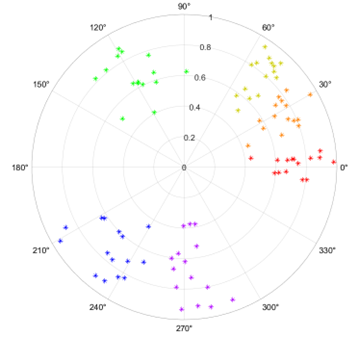
\includegraphics[width=0.9\columnwidth]{hsv_polar.png}}
    \hfil
    \caption{MATLAB~\cite{matlab} plot of training data HSV hues \( \left(\theta\right) \) and saturations \( \left(r\right) \) in polar form, colored by classification.}%
    \label{hsv_polar}
\end{figure}

A small test set of 18 colors (three per classification) was collected and saved in both RGB and
HSV formats. The training and test data for both RGB and HSV were then fed into the k-nearest
neighbor algorithm at k=3 and k=5, with the results shown in Table~\ref{rgb_knn_3}~to~\ref{hsv_knn_5}.
An example program output is shown in Appendix~\ref{program_demo}. With the given test data, the HSV data
was classified with a perfect success rate, as was the RGB data at k=3. The RGB data misclassified
one orange color as yellow at k=5, but the success rate was still high at 94\%. Given that both
the RGB and HSV data could be accurately classified by the k-nearest neighbor algorithm, both data
sets were tested in the other algorithms.

\begin{table*}[!t]
    \centering

    \begin{minipage}{\columnwidth}
        \centering
        \caption{RGB Bayesian classification results.}%
        \label{rgb_bayes}
        \begin{tabular}{ l l l l }
            \toprule
            \bfseries Color & \bfseries Classified & \bfseries Misclassified & \bfseries Success Rate \\
            \midrule
            Red             & 3                    & 0                       & 1.00                   \\
            Orange          & 2                    & 1 (1 yellow)            & 0.67                   \\
            Yellow          & 2                    & 1 (1 orange)            & 0.67                   \\
            Green           & 3                    & 0                       & 1.00                   \\
            Blue            & 3                    & 0                       & 1.00                   \\
            Purple          & 3                    & 0                       & 1.00                   \\
            \midrule
            \bfseries Total & \bfseries 16         & \bfseries 2             & \bfseries 0.89         \\
            \bottomrule
        \end{tabular}
    \end{minipage}%
    %
    \begin{minipage}{\columnwidth}
        \centering
        \caption{HSV Bayesian classification results.}%
        \label{hsv_bayes}
        \begin{tabular}{ l l l l }
            \toprule
            \bfseries Color & \bfseries Classified & \bfseries Misclassified & \bfseries Success Rate \\
            \midrule
            Red             & 0                    & 3 (2 orange, 1 purple)  & 0.00                   \\
            Orange          & 2                    & 1 (1 yellow)            & 0.67                   \\
            Yellow          & 3                    & 0                       & 1.00                   \\
            Green           & 2                    & 1 (1 red)               & 0.67                   \\
            Blue            & 3                    & 0                       & 1.00                   \\
            Purple          & 3                    & 0                       & 1.00                   \\
            \midrule
            \bfseries Total & \bfseries 13         & \bfseries 5             & \bfseries 0.72         \\
            \bottomrule
        \end{tabular}
    \end{minipage}
\end{table*}

From there, both data sets were tested in the Bayesian linear classifier, the results of which
are shown in Table~\ref{rgb_bayes}~and~\ref{hsv_bayes}.

Since the Bayesian algorithm relies on means, the HSV data set performs poorly, as the red's hue
wrapping at 360 is not handled correctly. This can be resolved by mapping the data points to the
complex plane. Doing so requires adjustments to the Bayesian algorithm:
\begin{itemize}
    \item The means used by the algorithm need to be the conjugate of the training data means.
          This way, when a test data point closely matches the classification, \( e^{i\theta} * e^{-i\theta} = 1 \),
          so the real component of the dot product can be used to determine classification.

    \item The mean offset \( \mu_0 \) needs to be calculated by taking the dot product of the means vector
          with the conjugate means vector, eliminating complex values from the offset.
\end{itemize}

\begin{table}[!t]
    \centering

    \caption{Complex HSV Bayesian classification results.}%
    \label{hsv_complex_bayes}
    \begin{tabular}{ l l l l }
        \toprule
        \bfseries Color & \bfseries Classified & \bfseries Misclassified & \bfseries Success Rate \\
        \midrule
        Red             & 3                    & 0                       & 1.00                   \\
        Orange          & 2                    & 1 (1 yellow)            & 0.67                   \\
        Yellow          & 3                    & 0                       & 1.00                   \\
        Green           & 3                    & 0                       & 1.00                   \\
        Blue            & 3                    & 0                       & 1.00                   \\
        Purple          & 3                    & 0                       & 1.00                   \\
        \midrule
        \bfseries Total & \bfseries 17         & \bfseries 1             & \bfseries 0.94         \\
        \bottomrule
    \end{tabular}
\end{table}

\begin{table*}[!b]
    \centering

    \begin{minipage}{\columnwidth}
        \centering
        \caption{RGB binary SLP classification results, \( \eta = 1 \).}%
        \label{rgb_binary_slp}
        \begin{tabular}{ l l l l }
            \toprule
            \bfseries Color & \bfseries Classified & \bfseries Misclassified & \bfseries Success Rate \\
            \midrule
            Red             & 3                    & 0                       & 1.00                   \\
            Green           & 3                    & 0                       & 1.00                   \\
            \midrule
            \bfseries Total & \bfseries 6          & \bfseries 0             & \bfseries 1.00         \\
            \bottomrule
        \end{tabular}
    \end{minipage}%
    %
    \begin{minipage}{\columnwidth}
        \centering
        \caption{Complex HSV binary SLP classification results, \( \eta = 1 \).}%
        \label{hsv_binary_slp}
        \begin{tabular}{ l l l l }
            \toprule
            \bfseries Color & \bfseries Classified & \bfseries Misclassified & \bfseries Success Rate \\
            \midrule
            Red             & 3                    & 0                       & 1.00                   \\
            Green           & 3                    & 0                       & 1.00                   \\
            \midrule
            \bfseries Total & \bfseries 6          & \bfseries 0             & \bfseries 1.00         \\
            \bottomrule
        \end{tabular}
    \end{minipage}
\end{table*}

The data was then converted to complex HSV values and run through the Bayesian classifier, the
results of which are shown in Table~\ref{hsv_complex_bayes}. This results in more reasonable classifications, so the
complex HSV values were used instead of the regular HSV values in the remaining algorithms.

For both the RGB data in Table~\ref{rgb_bayes} and the complex HSV data in Table~\ref{hsv_complex_bayes}, the Bayesian
classifier achieved a high success rate (89\% and 94\%, respectively), but there is still room for
improvement given the success rate of the k-nearest neighbor algorithm. As a result, the single-layer
perceptron algorithm was tested on both data sets.

Before running a multiclass SLP algorithm, however, a subset of the data was run through a standard, binary class SLP algorithm to test the behavior of
the system.

Just like with the Bayesian algorithm, the SLP algorithm requires adjustments to support
complex numbers:

\begin{itemize}
    \item When training the weights, the conjugates of the training data point components are used
          to adjust the weight. Once again, this makes it so data points that match the classification
          are rotated towards a real value of 1, strengthening its classification value.

    \item When running the classifier on test data, the real component of the calculated
          classification value is used to determine classification.
\end{itemize}

The red and green classifications were chosen for testing. While testing the data, it was observed
that the weights would occasionally fail to converge or oscillate around convergence. After
adjusting the algorithm to subtract the mean of the entire testing data set from all data points, the
behavior improved significantly. The results of the algorithm are shown in Table~\ref{rgb_binary_slp}~and~\ref{hsv_binary_slp}.

As can be seen with the complex HSV data, the adjustments to account for complex numbers
were successful. Additionally, all data was successfully classified, so it was worth proceeding with
the multiclass SLP algorithm.

Compared to the binary SLP algorithm, the multiclass SLP algorithm stores multiple weight vectors---one
for each classification---and utilizes the ``one-vs.-rest''~\cite{bishop} method of training the
weights. While training, the data point is tested against all the weight vectors, and the
classification with the largest calculated value is assigned to the data point. If the classification is
correct, then the weights are not adjusted. Otherwise, the weights of the correct class are
increased by adding \( \eta\left(k\right)\mathbf{y}_k \), where \( \eta\left(k\right) \) is the learning
rate and \( \mathbf{y}_k \) is the training data point, and the weights of the other classes are decreased
by subtracting that same value. When testing data against the weights, whichever classification has the
largest calculated value is assigned to the data point.

Once again, the algorithm requires adjustments to support complex numbers:
\begin{itemize}
    \item When training the weights, the conjugates of the data point components are used to adjust
          the weight.

    \item The real component of the calculated classification value is used to determine the
          classification of data points.
\end{itemize}

\begin{table*}[!t]
    \centering

    \begin{minipage}{\columnwidth}
        \centering
        \caption{RGB multiclass SLP classification results, \( \eta = 1 \).}%
        \label{rgb_slp}
        \begin{tabular}{ l l l l }
            \toprule
            \bfseries Color & \bfseries Classified & \bfseries Misclassified & \bfseries Success Rate \\
            \midrule
            Red             & 9                    & 0                       & 1.00                   \\
            Orange          & 8                    & 1 (1 yellow)            & 0.89                   \\
            Yellow          & 9                    & 0                       & 1.00                   \\
            Green           & 8                    & 1 (1 yellow)            & 0.89                   \\
            Blue            & 9                    & 0                       & 1.00                   \\
            Purple          & 9                    & 0                       & 1.00                   \\
            \midrule
            \bfseries Total & \bfseries 52         & \bfseries 2             & \bfseries 0.96         \\
            \bottomrule
        \end{tabular}
    \end{minipage}%
    %
    \begin{minipage}{\columnwidth}
        \centering
        \caption{Complex HSV multiclass SLP classification results, \( \eta = 1 \).}%
        \label{hsv_slp}
        \begin{tabular}{ l l l l }
            \toprule
            \bfseries Color & \bfseries Classified & \bfseries Misclassified & \bfseries Success Rate \\
            \midrule
            Red             & 9                    & 0                       & 1.00                   \\
            Orange          & 9                    & 0                       & 1.00                   \\
            Yellow          & 9                    & 0                       & 1.00                   \\
            Green           & 9                    & 0                       & 1.00                   \\
            Blue            & 9                    & 0                       & 1.00                   \\
            Purple          & 9                    & 0                       & 1.00                   \\
            \midrule
            \bfseries Total & \bfseries 54         & \bfseries 0             & \bfseries 1.00         \\
            \bottomrule
        \end{tabular}
    \end{minipage}
\end{table*}

The results of running the multiclass SLP algorithm are shown in Table~\ref{rgb_slp}~and~\ref{hsv_slp}. Each test was
run three times to account for the initial random state of the weights.

For both the RGB and the complex HSV data sets, the multiclass SLP classifier shows a
significantly better classification rate for the given training and test data than the Bayesian
classifier. Additionally, the complex HSV data set has a perfect success rate with the given
classifications.

\section{Conclusion}

Looking at the results in Table~\ref{rgb_slp}~and~\ref{hsv_slp}, the multiclass SLP algorithm is an accurate and efficient
method of classifying colors. Comparing the multiclass SLP results to those of the Bayesian
algorithm in Table~\ref{rgb_bayes}~and~\ref{hsv_complex_bayes}, it is safe to assume that in the general use case, color data's class
conditional density functions do not perfectly follow a Gaussian distribution~\cite{farmer}. Additionally,
comparing the results of Table~\ref{rgb_slp}~and~\ref{hsv_slp} show that mapping RGB colors to complex HSV
colors can result in better linear classification.

One issue with the implementation of the SLP algorithms in this paper is that the algorithm often
falls into a local minimum. Because of the random starting weights, the algorithm is not
guaranteed to find the absolute minimum, resulting in the algorithm varying in accuracy each
time it is retrained. This was observed with the RGB multiclass results in Table~\ref{rgb_slp}; one run
classified everything perfectly, while the other two each misclassified one different data point.
This can be improved by adding momentum to the weight adjustments during training.

There is also room for further research on the accuracy of classification using RGB colors vs.
complex HSV colors. The classifications used in this paper strongly lined up with hue, but it is
possible that a different classification system, such as differentiating between several types of
blue, will perform better using RGB than with HSV.\@

\appendices%

\section{Plots of Training Data}%
\label{train_data_plots}

\begin{figure*}[!b]
    \centering
    \subfloat{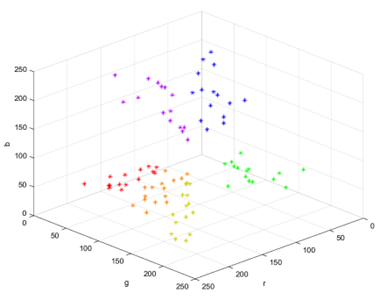
\includegraphics[width=\columnwidth]{rgb_isometric.png}}
    \hfill
    \subfloat{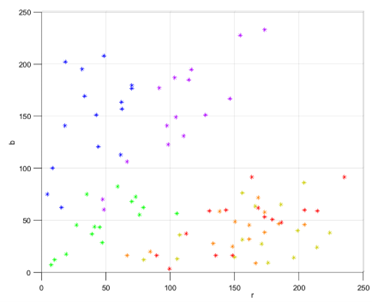
\includegraphics[width=\columnwidth]{rgb_front.png}}
    \hfill
    \subfloat{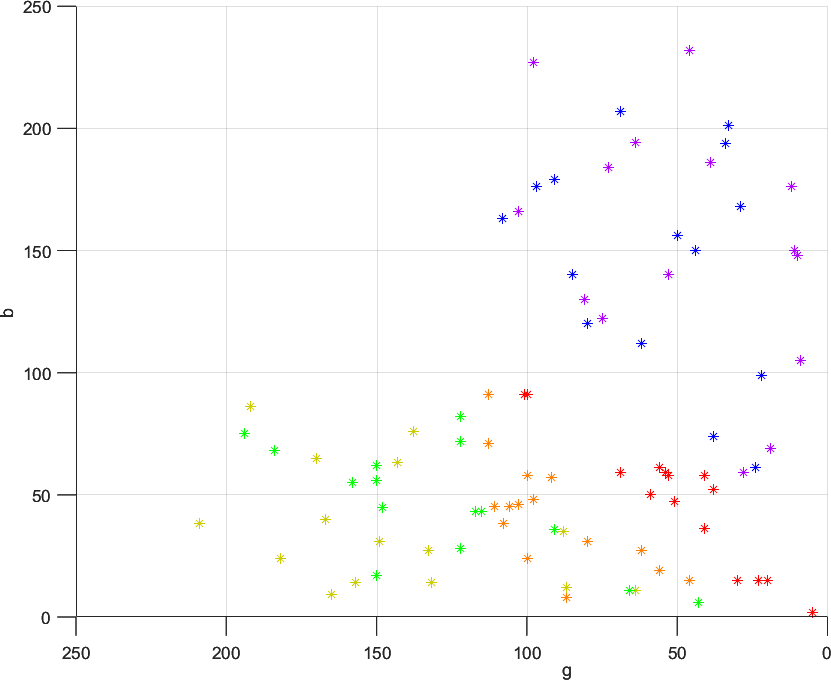
\includegraphics[width=\columnwidth]{rgb_left.png}}
    \hfill
    \subfloat{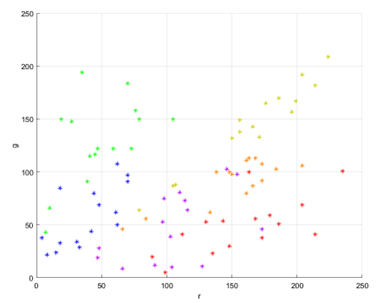
\includegraphics[width=\columnwidth]{rgb_top.png}}
    \hfill
    \caption{MATLAB~\cite{matlab} plot of training data RGB values, colored by classification.}%
    \label{rgb_data}
\end{figure*}

\begin{figure*}[!t]
    \centering
    \subfloat{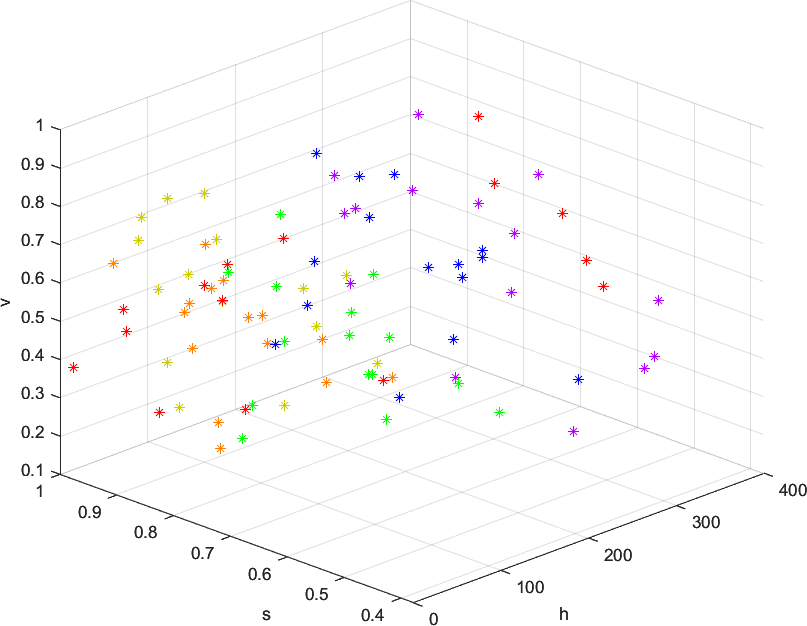
\includegraphics[width=\columnwidth]{hsv_isometric.png}}
    \hfill
    \subfloat{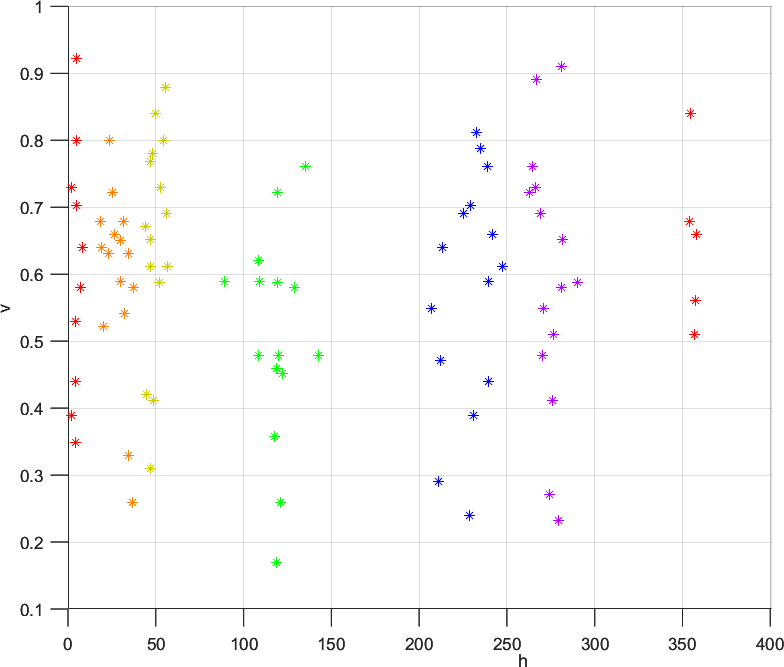
\includegraphics[width=\columnwidth]{hsv_front.png}}
    \hfill
    \subfloat{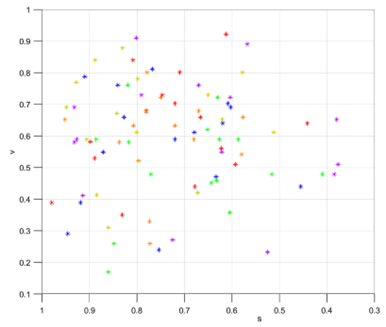
\includegraphics[width=\columnwidth]{hsv_left.png}}
    \hfill
    \subfloat{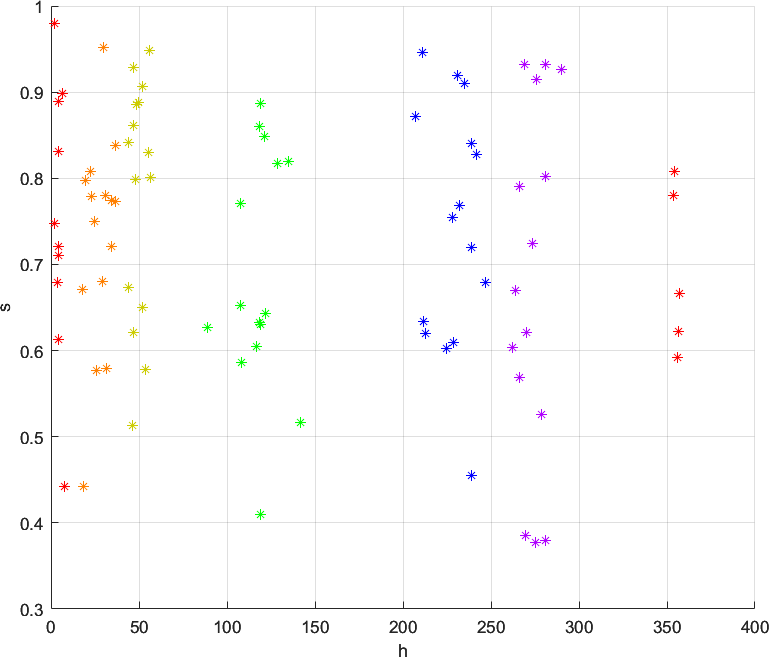
\includegraphics[width=\columnwidth]{hsv_top.png}}
    \hfill
    \caption{MATLAB~\cite{matlab} plot of training data HSV values, colored by classification.}%
    \label{hsv_data}
\end{figure*}

Fig.~\ref{rgb_data} shows plots of the RGB training data, and Fig.~\ref{hsv_data} shows
plots of the HSV training data.

\section{Program Demonstration}%
\label{program_demo}

Fig.~\ref{program_output} shows an example of the output from running the multiclass SLP program.

\begin{figure*}[!t]
    \centering
    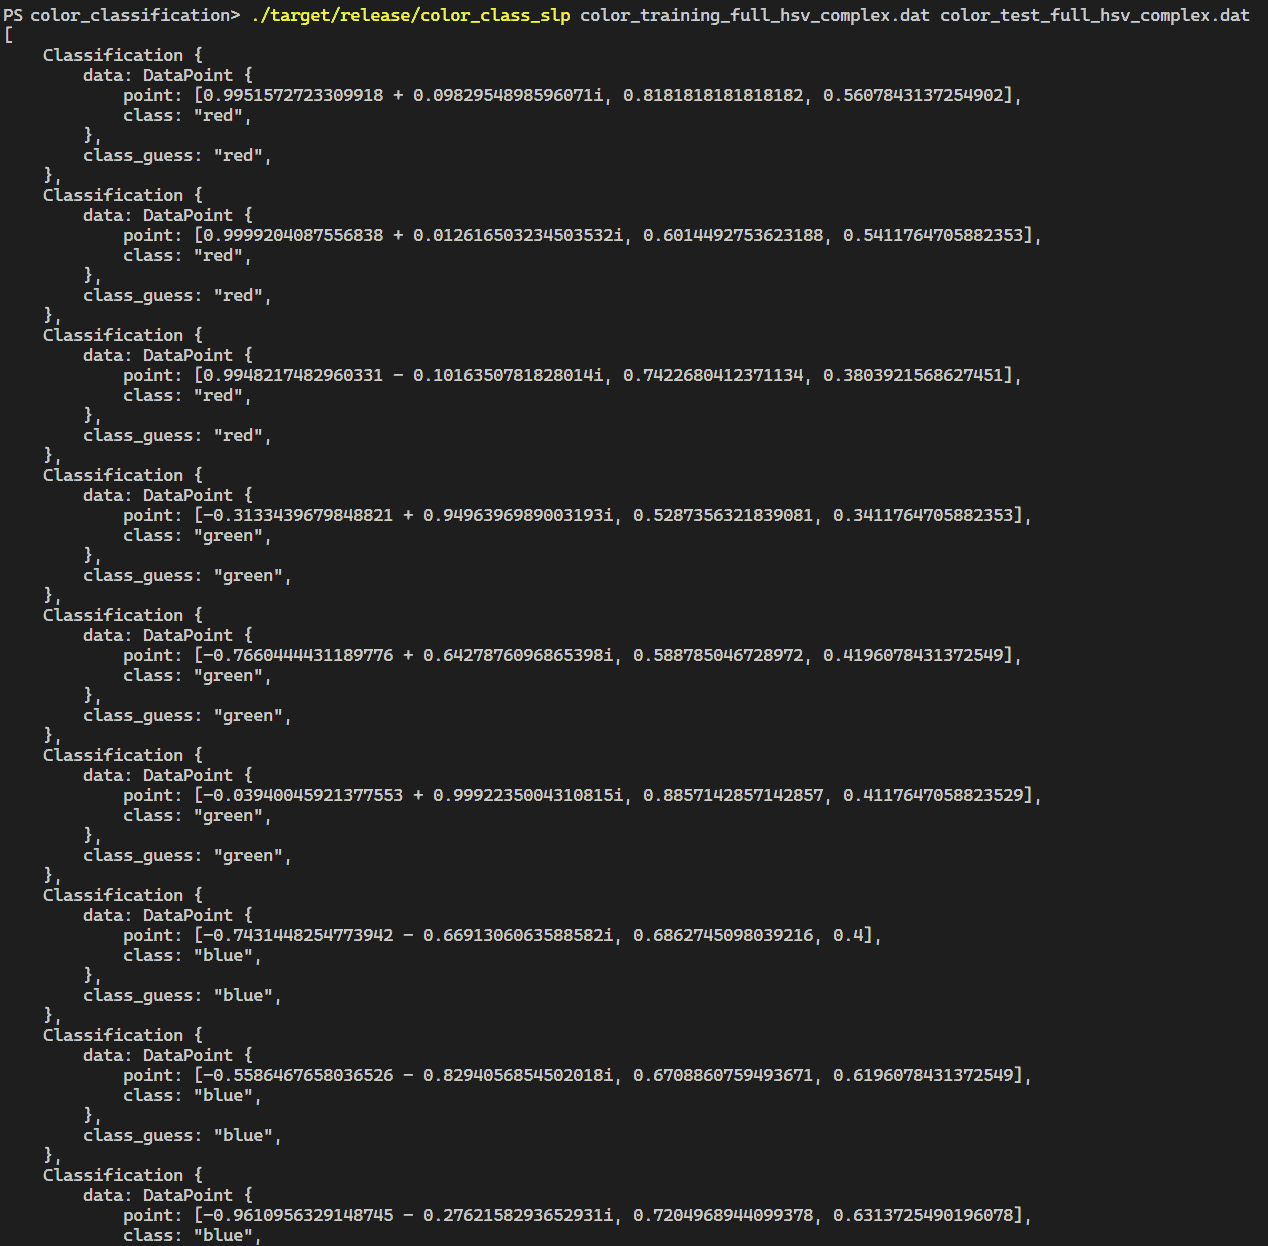
\includegraphics[width=0.75\textwidth]{program_demo.png}
    \hfil
    \caption{Example program output of the multiclass SLP using complex HSV colors.}%
    \label{program_output}
\end{figure*}

\section{Program Source Code and Data Files}%
\label{program_source}

The data in this study is plotted in MATLAB~\cite{matlab}, and the algorithms are written in Rust.
The source code and data files are available in \mbox{benjamin\_hall\_color\_classification.zip}.

The data files used in the algorithms are as follows:
\begin{itemize}
    \item k-nearest neighbor
          \begin{itemize}
              \item RGB
                    \begin{itemize}
                        \item color\_training\_full.dat
                        \item color\_test\_full.dat
                    \end{itemize}
              \item HSV
                    \begin{itemize}
                        \item color\_training\_full\_hsv.dat
                        \item color\_test\_full\_hsv.dat
                    \end{itemize}
          \end{itemize}

    \item Bayesian
          \begin{itemize}
              \item RGB
                    \begin{itemize}
                        \item color\_training\_full.dat
                        \item color\_test\_full.dat
                    \end{itemize}
              \item HSV
                    \begin{itemize}
                        \item color\_training\_full\_hsv.dat
                        \item color\_test\_full\_hsv.dat
                    \end{itemize}
              \item Complex HSV
                    \begin{itemize}
                        \item color\_training\_full\_hsv\_complex.dat
                        \item color\_test\_full\_hsv\_complex.dat
                    \end{itemize}
          \end{itemize}

    \item Binary SLP
          \begin{itemize}
              \item RGB
                    \begin{itemize}
                        \item color\_training\_binary.dat
                        \item color\_test\_binary.dat
                    \end{itemize}
              \item Complex HSV
                    \begin{itemize}
                        \item color\_training\_binary\_hsv\_complex.dat
                        \item color\_test\_binary\_hsv\_complex.dat
                    \end{itemize}
          \end{itemize}

    \item Multiclass SLP
          \begin{itemize}
              \item RGB
                    \begin{itemize}
                        \item color\_training\_full.dat
                        \item color\_test\_full.dat
                    \end{itemize}
              \item Complex HSV
                    \begin{itemize}
                        \item color\_training\_full\_hsv\_complex.dat
                        \item color\_test\_full\_hsv\_complex.dat
                    \end{itemize}
          \end{itemize}
\end{itemize}

\enlargethispage{-1.15in}

\bibliographystyle{IEEEtran}
\bibliography{IEEEabrv,refs}

\end{document}
